\documentclass[9pt,twocolumn,twoside,]{pnas-new}

%% Some pieces required from the pandoc template
\providecommand{\tightlist}{%
  \setlength{\itemsep}{0pt}\setlength{\parskip}{0pt}}

% Use the lineno option to display guide line numbers if required.
% Note that the use of elements such as single-column equations
% may affect the guide line number alignment.


\usepackage[T1]{fontenc}
\usepackage[utf8]{inputenc}


\templatetype{pnasresearcharticle}  % Choose template

\title{Parsing medial prefrontal cortex: A joint meta-analytic and
graph-theoretic approach.}

\author[a,1,2]{Claudio A. Toro-Serey}
\author[a,1]{Joseph T. McGuire}

  \affil[a]{Boston University, Department of Psychological and Brain Sciences, 64
Commonwealth Ave., Boston, 02250}


% Please give the surname of the lead author for the running footer
\leadauthor{Toro-Serey}

% Please add here a significance statement to explain the relevance of your work
\significancestatement{Authors must submit a 120-word maximum statement about the significance
of their research paper written at a level understandable to an
undergraduate educated scientist outside their field of speciality. The
primary goal of the Significance Statement is to explain the relevance
of the work in broad context to a broad readership. The Significance
Statement appears in the paper itself and is required for all research
papers.}


\authorcontributions{Please provide details of author contributions here.}

\authordeclaration{Please declare any conflict of interest here.}

\equalauthors{\textsuperscript{} }

\correspondingauthor{\textsuperscript{} }

% Keywords are not mandatory, but authors are strongly encouraged to provide them. If provided, please include two to five keywords, separated by the pipe symbol, e.g:
 \keywords{  Networks |  DMN |  Valuation   }

\begin{abstract}
(Current count: 153) Valuation effects are consistently observed in
medial prefrontal and posterior cingulate cortex (mPFC and PCC). The
spatial extent of these effects is mostly indistinguishable from the
default mode network (DMN) in existing meta-analyses. However, little is
known about how valuation effects fit within the broader functional
architecture of mPFC and PCC, or whether that architecture is consistent
or idiosyncratic across individuals. Here we complement a meta-analysis
with fMRI-based graph theoretic approaches to subdivide mPFC and PCC at
the single-subject level. Our results suggest the functional topography
of mPFC has substantial variability across individuals. This highlights
the potential usefulness of estimating brain effects at the individual
level in this region, and points to limitations of aggregative methods
such as coordinate-based meta-analysis in determining whether valuation
and DMN effects emerge from common or separable brain systems. Our
approach shows promise in addressing this issue through future
manipulations of valuation.
\end{abstract}

\dates{This manuscript was compiled on \today}
\doi{\url{www.pnas.org/cgi/doi/10.1073/pnas.XXXXXXXXXX}}

\begin{document}

% Optional adjustment to line up main text (after abstract) of first page with line numbers, when using both lineno and twocolumn options.
% You should only change this length when you've finalised the article contents.
\verticaladjustment{-2pt}

\maketitle
\thispagestyle{firststyle}
\ifthenelse{\boolean{shortarticle}}{\ifthenelse{\boolean{singlecolumn}}{\abscontentformatted}{\abscontent}}{}

% If your first paragraph (i.e. with the \dropcap) contains a list environment (quote, quotation, theorem, definition, enumerate, itemize...), the line after the list may have some extra indentation. If this is the case, add \parshape=0 to the end of the list environment.

\acknow{Please include your acknowledgments here, set in a single paragraph.
Please do not include any acknowledgments in the Supporting Information,
or anywhere else in the manuscript.}

(current, 676 words. Aim for 650)

The medial prefrontal cortex (mPFC) has been suggested to subserve many
of the cognitive abilities that differentiate humans from other animals
(Barbas \& Garcia-Cabezas, 2016). Specifically, this region has been
related to decision making (Bartra, McGuire, \& Kable, 2013), memory
encoding (Shacter, Addis, \& Buckner, 2007), and default mode
deactivation (DMN) (Yeo et al., 2011), among ohters. While much has been
discovered about this area in primates (Barbas \& Garcia-Cabezas, 2016),
the lack of direct measurements of neuronal activity makes this a tough
area to record in humans, one that nowadays relies mostly on functional
MRI (fMRI). Unfortunately, the mPFC is especially challenging to image,
as the oxygen-related signal recorded by fMRI is contaminated by the
oxygen in the sinuses (Logothetis, 2008). In addition, this area is
subject to more idiosyncratic cortical folding than any other region
(Zilles, Palomero- Gallagher, \& Amunts, 2013), thus adding a level of
complexity to the generalizable dissection of topographic functional
roles within mPFC.

Previous meta analytic studies have provided important insights on the
psychological phenomena attributed to mPFC subregions. For example, de
la Vega et al. (2016) found subdivisions of mPFC and MCC that are
significantly tied to decision making in the literature. In particular,
they show that more ventral regions are more tightly associated with
reward and fear. However, this pattern overlaps with their finding that
vmPFC also coactivates with DMN regions, and find no topographical
distinction between these phenomena. Similarly, the results from Bartra
et al and Laird et al show that this region can't be subdivided into DMN
vs subjective value (acikalin, chris, russ). However, meta analyses rely
on peaks often derived from group-averaged data. Recent work has
prescribed relevance to the analysis of single subjects in fMRI. Yeo et
al (2018) propose the use of individualized topologies when identifying
functional networks. Gordon et al identify important idiosincrasies in
oversampled subjects. Similarly, Braga and Buckner show that finer
subdivisions of the DMN are possible when looking at each subject
independently. This opens up the possibility that distinctions between
DMN and subjective value are possible at this finer level of resolution,
but would otherwise be masked in meta analytic work.

Braga \& Buckner's work is particularly informative when it comes to
subdividing DMN. However, the seed-based functional connectivity
analysis is sensitive to the selection of the seed. A natural next step
would be to recruit all possible patterns of covariation within this
network. A popular alternative is to rely on graph theoretic methods,
which provide a characterization of networks that organically fits brain
dynamics (provides an organic avenue to understand brain dynamics?), and
thus permits the consideration of the full covariance structure of brain
networks. (ADV \& Tal somewhere here).

Given the shortcomings of study-specific and cross-study analyses
mentioned above, there is potential value in combining complementary
strengths from both approaches. Focusing on resting state data has been
successful in determining a number of neural phenomena, including
disentangling auditory and visual attention areas (Tobyne, Osher,
Michalka, \& Somers, 2017).

One great advantage of network science is the ability to characterize
connectivity in a way that allows for comparisons among individuals in a
meaningful way (Garcia, Ashourvan, Muldoon, Vettel, \& Bassett, 2018),
thus letting us address the idiosyncrasies mentioned above. In this
study, we aim to subdivide mPFC into subject-specific DMN and non-DMN
areas, so that we can generate more informed topographic targets for
future studies of decision making. We address this aim at 3 levels of
granularity: 1) across the literature (meta-analysis), selecting a
number of regions of interest (ROI) that show significant overlap and
specificity between DMN and decision making; 2) full-brain connectivity
of actual fMRI data, using a pre-specified brain atlas; and 3)
characterizing the connectivity of surface vertices (small units of
function that contain oxygen-dependent neural information across time)
for the regions selected in step one. I performed the last two steps at
an individual subject level for 3 subjects, hoping to find some
commonalities among them. In this way, I attempted to extract functional
topographical information from topological network features.

\section*{Results}\label{results}
\addcontentsline{toc}{section}{Results}

\begin{figure}
\centering
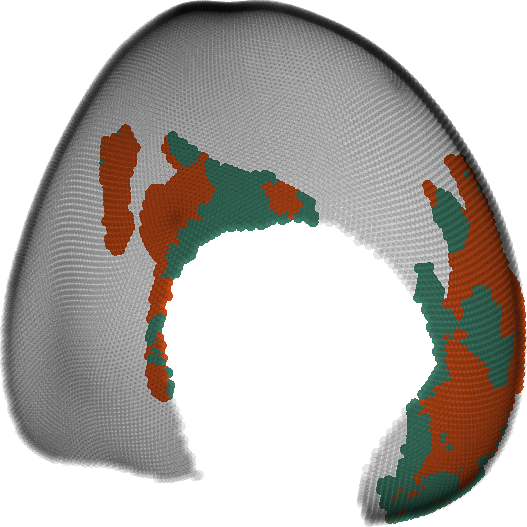
\includegraphics{Manuscript_files/figure-latex/Partition comparison: all brain example-1.pdf}
\caption{Template brain.}
\end{figure}

\section*{Discussion}\label{discussion}
\addcontentsline{toc}{section}{Discussion}

(1500 words max)

\section*{Methods}\label{methods}
\addcontentsline{toc}{section}{Methods}

See \url{http://www.jneurosci.org/content/preparing-manuscript}

\textbf{Meta-analysis} To perform the first step, I used data from a
metanalysis that gathered peak brain coordinates of activity from
studies of valuation (n = 27 studies) and DMN (n = 77). These are the
surviving areas post-statistical thresholding from each study. I
analyzed this data by mapping the peak cortical coordinates to an atlas
of the human cortical surface (Glasser et al., 2016). This produced a
list of standardized parcels that were reported on each study. The
advantage of utilizing this atlas was threefold: first, it reduced the
number of functional vertices from 60,000 (cortical surface vertices) to
360 (cortical parcels). Second, it standardizes the vertices from the
first to the second stage of my study. Finally, it allowed me to project
each area on a brain space without much clutter. Since each vertex is
embedded with topographical information, and since functional topography
is essential to my question, I mostly project my results onto brain
space.

I thus generated two undirected, loop-less, weighted graphs in which
each vertex was a brain parcel, and edges correspond to the number of
times each pair of them co-occurred across studies. Since different
decision tasks use different sensory modalities, and since sensory areas
get sometimes reported as unrelated peak coordinates in DMN studies, I
bootstrapped the co- occurrences across studies and removed edges whose
co-occurrences lied below the 90th percentile. Based on this, only edges
with co-occurrences higher than 8 were preserved, and the remaining
unconnected vertices (brain regions) were discarded. With these graphs
set up, I computed the strength and betweenness centrality in order to
capture each parcel's centrality in the valuation and DMN literatures
separately.

In order to select of regions of interest (ROI) from mPFC and other
brain areas that are central to valuation and DMN literatures, I first
bootstrapped the mean strength for each graph separately, and chose
areas with strength above the 95th percentile of this distribution.
Next, I took the intersection of these areas, such that the final ROIs
were brain regions that overlapped between DMN and valuation in the
literature (and thus my main target for dissociation).

\textbf{Whole Brain Parcellated connectivity} For the second step, in
order to actually quantify the intrinsic connectivity of these ROIs in
the brain, I used data from the Human Connectome Project. Specifically,
I acquired resting-state fMRI activity from 3 subjects, all of whom have
been preprocessed according to industry standards to allow for
group-level comparisons (Tobyne et al., 2017). Each data set contained
around 1 hour of signals represented as 4800 time points, and each
subject contained 60,000 vertices. I parcellated each subject's brain
according to the atlas mentioned above, so that each parcel contained
the mean time series from its vertices, and correlated the mean time
series among all parcels (Pearson). This produced a weighted adjacency
matrix for each subject, where each of the 360 parcels is a vertex, and
edges the correlations among all of them. Next, I took the exponential
of the correlations, Fisher transformed them (i.e.~tanh) so that all
weights were positive while maintaining the shape of the original
correlation distribution, and retained the edges whose adjusted p-values
remained significant (FDR \textless{} 0.05). Again, I quantified each
parcel's strength and betweenness, averaged them across subjects, and
examined whether any of the ROIs showed uniquely high centralities. For
this, I performed a permutation comparing the mean strength between the
ROIs and the rest of the brain for each participant.

For the main goal of this section, I maximized the strength-based
modularity metric as a community detection method (fast-greedy
algorithm), so that I could check if all the DMN ROIs from the previous
section were affiliated with the same community. While this measure has
resolution problems at large and low scales (Fortunato \& Hric, 2016),
if it does extract a close match to standard DMN networks, it could act
as a good method for the final stage of the project (but see Peel,
Larremore, and Clauset 2017 for issues with ground-truth). Even though
this analysis is mainly geared to confirm that these ROIs are jointly
captured, this step also let me examine whether some of the ROIs could
be subdivided into DMN and non-DMN regions at this level of granularity.

In order to evaluate the validity of the modularity-based communities, I
also clustered the brain by means of spectral partitioning.
Specifically, I took the Fiedler vector (eigenvector associated with the
second lowest eigenvalue) from each participant's normalized Laplacian
matrix, and divided the brain by the sign of the eigenvector values.
This analysis served the additional purpose of more strictly dividing
the brain into DMN and non-DMN communities. Importantly, given the high
density of these networks (see results), spectral partitioning was
unlikely to face the issues associated with its use in sparse networks
(Fortunato \& Hric, 2016). Finally, to quantify the agreement of these
community methods, I computed both the adjusted rand index and variation
of information distance (normalized by the logarithm of the number of
vertices, 360 in this case) between them per subject. The adjusted rand
index denotes the proportion of vertices that coincide in affiliation
across partitions, and compares this score to a baseline given by the
expectation based on a random vertex assignment for an equal number of
clusters across partitions. On the other hand, variation of information
gives a general sense of the amount of information to be gained by the
complementary community partitioning (Meila, 2007), measured by the
addition of the conditional entropies per combination of clusters across
partitions. While the rand index is more easily interpreted, it suffers
from the assumption that the baseline should have an equal number of
vertices per cluster across partitions, which is not necessarily the
case. Therefore, I used variation of information as a more robust
similarity metric (Fortunato \& Hric, 2016). Importantly, due to having
just 3 subjects, I abstained from performing formal statistics on the
descriptive measures that I show.

\textbf{Within-ROI Connectivity} For the third stage, I ``zoomed in''
each subject's brain by computing the correlation among all of the
surface-vertices contained within each ROI across all the ROIs, and
applied the same correction as in step two. That means that the vertices
became smaller functional brain units that are connected by the same
type of edge (i.e.~adjusted correlations) as in step two. This time, I
only focused on partitioning the brain through modularity and spectral
partitioning to see if the ROIs can be subdivided at this finer level of
resolution. It is worth noting that while communities across subjects
should be similar, the idiosyncrasies explained previously
(i.e.~cortical folding) should produce noticeable differences as well.

This time I added two new areas to the ROIs: 7m, as this area had unique
relevance in DMN when compared to valuation (evidenced by its
connectivity strength in DMN and chi- squared permutation in the
meta-analysis, see results), and V1, as this visual processing area
should not be affiliated with DMN. These regions thus acted as dual
reference points, such that the community affiliated with 7m should
denote DMN, while V1 indicated non-DMN. As before, I tested the validity
of the partitions using the adjusted rand index and normalized variation
of information. However, this time I also used the rand index to
quantify the community correspondence between subjects. Specifically, I
divided each subject's spectrally- partitioned brain into PCC and mPFC
topographical zones (posterior and frontal brain, respectively), and
computed the index of each region between subjects. The high
cross-subject heterogeneity of cortical folding of mPFC should produce
relatively low rand indices, while the more homogeneous PCC should
display the opposite pattern. This analysis was meant to tackle the
subject-specific limitations discussed above. The final patterns were
inspected visually.

\section*{References}\label{references}
\addcontentsline{toc}{section}{References}

Figures and Tables should be labelled and referenced in the standard way
using the \texttt{\textbackslash{}label\{\}} and
\texttt{\textbackslash{}ref\{\}} commands.

Figure \[fig:frog\] shows an example of how to insert a column-wide
figure. To insert a figure wider than one column, please use the
\texttt{\textbackslash{}begin\{figure*\}...\textbackslash{}end\{figure*\}}
environment. Figures wider than one column should be sized to 11.4 cm or
17.8 cm wide.

\subsection*{Single column equations}\label{single-column-equations}
\addcontentsline{toc}{subsection}{Single column equations}

Authors may use 1- or 2-column equations in their article, according to
their preference.

To allow an equation to span both columns, options are to use the
\texttt{\textbackslash{}begin\{figure*\}...\textbackslash{}end\{figure*\}}
environment mentioned above for figures, or to use the
\texttt{\textbackslash{}begin\{widetext\}...\textbackslash{}end\{widetext\}}
environment as shown in equation \[eqn:example\] below.

Please note that this option may run into problems with floats and
footnotes, as mentioned in the \href{http://texdoc.net/pkg/cuted}{cuted
package documentation}. In the case of problems with footnotes, it may
be possible to correct the situation using commands
\texttt{\textbackslash{}footnotemark} and
\texttt{\textbackslash{}footnotetext}.

\[\begin{aligned}
(x+y)^3&=(x+y)(x+y)^2\\
       &=(x+y)(x^2+2xy+y^2) \label{eqn:example} \\
       &=x^3+3x^2y+3xy^3+x^3. 
\end{aligned}\]

\subsection*{Supporting Information
(SI)}\label{supporting-information-si}
\addcontentsline{toc}{subsection}{Supporting Information (SI)}

The main text of the paper must stand on its own without the SI. Refer
to SI in the manuscript at an appropriate point in the text. Number
supporting figures and tables starting with S1, S2, etc. Authors are
limited to no more than 10 SI files, not including movie files. Authors
who place detailed materials and methods in SI must provide sufficient
detail in the main text methods to enable a reader to follow the logic
of the procedures and results and also must reference the online
methods. If a paper is fundamentally a study of a new method or
technique, then the methods must be described completely in the main
text. Because PNAS edits SI and composes it into a single PDF, authors
must provide the following file formats only.

\subsubsection*{SI Text}\label{si-text}
\addcontentsline{toc}{subsubsection}{SI Text}

Supply Word, RTF, or LaTeX files (LaTeX files must be accompanied by a
PDF with the same file name for visual reference).

\subsubsection*{SI Figures}\label{si-figures}
\addcontentsline{toc}{subsubsection}{SI Figures}

Provide a brief legend for each supporting figure after the supporting
text. Provide figure images in TIFF, EPS, high-resolution PDF, JPEG, or
GIF format; figures may not be embedded in manuscript text. When saving
TIFF files, use only LZW compression; do not use JPEG compression. Do
not save figure numbers, legends, or author names as part of the image.
Composite figures must be pre-assembled.

\subsubsection*{3D Figures}\label{d-figures}
\addcontentsline{toc}{subsubsection}{3D Figures}

Supply a composable U3D or PRC file so that it may be edited and
composed. Authors may submit a PDF file but please note it will be
published in raw format and will not be edited or composed.

\subsubsection*{SI Tables}\label{si-tables}
\addcontentsline{toc}{subsubsection}{SI Tables}

Supply Word, RTF, or LaTeX files (LaTeX files must be accompanied by a
PDF with the same file name for visual reference); include only one
table per file. Do not use tabs or spaces to separate columns in Word
tables.

\subsubsection*{SI Datasets}\label{si-datasets}
\addcontentsline{toc}{subsubsection}{SI Datasets}

Supply Excel (.xls), RTF, or PDF files. This file type will be published
in raw format and will not be edited or composed.

\subsubsection*{SI Movies}\label{si-movies}
\addcontentsline{toc}{subsubsection}{SI Movies}

Supply Audio Video Interleave (avi), Quicktime (mov), Windows Media
(wmv), animated GIF (gif), or MPEG files and submit a brief legend for
each movie in a Word or RTF file. All movies should be submitted at the
desired reproduction size and length. Movies should be no more than 10
MB in size.

\subsubsection*{Still images}\label{still-images}
\addcontentsline{toc}{subsubsection}{Still images}

Authors must provide a still image from each video file. Supply TIFF,
EPS, high-resolution PDF, JPEG, or GIF files.

\subsubsection*{Appendices}\label{appendices}
\addcontentsline{toc}{subsubsection}{Appendices}

PNAS prefers that authors submit individual source files to ensure
readability. If this is not possible, supply a single PDF file that
contains all of the SI associated with the paper. This file type will be
published in raw format and will not be edited or composed.

\showmatmethods
\showacknow
\pnasbreak



% Bibliography
% \bibliography{pnas-sample}

\end{document}

